\documentclass[output=paper,colorlinks,citecolor=brown]{langscibook}
\ChapterDOI{10.5281/zenodo.15682196}
\title[Basic verb vocabulary: An empirical approach]{Basic verb vocabulary: An empirical approach to argument structure and word associations}

\author{Valentina Stefanova\orcid{0000-0003-3334-2050}\affiliation{Department of Computational Linguistics, Institute for Bulgarian Language, Bulgarian Academy of Sciences} and Maria A. Todorova\orcid{0000-0001-5866-7180}\affiliation{Department of Computational Linguistics, Institute for Bulgarian Language, Bulgarian Academy of Sciences} and Tsvetana Dimitrova\orcid{0000-0002-8972-435X}\affiliation{Department of Computational Linguistics, Institute for Bulgarian Language, Bulgarian Academy of Sciences}}

\abstract{The article discusses the results of a pilot survey on basic verb vocabulary conducted through an online experiment in the form of language tasks \editcolor{red}{employing associative stimuli, thematic stimuli, and contextual and textual stimuli. An analysis revolves around observations on the performance of the tasks by two focus groups of children -- 7- to 10-year-olds and 11- to 14-year-olds. Semantic frame representations of the selected verbs are employed to explain the specifics of the respondents' competence in recognising the selected verb meanings and the arguments associated with a specific verb meaning.}
}
\IfFileExists{../localcommands.tex}{
 \addbibresource{../localbibliography.bib}
 \usepackage{langsci-optional}
\usepackage{langsci-gb4e}
\usepackage{langsci-lgr}

\usepackage{listings}
\lstset{basicstyle=\ttfamily,tabsize=2,breaklines=true}

%added by author
% \usepackage{tipa}
\usepackage{multirow}
\graphicspath{{figures/}}
\usepackage{langsci-branding}

 
\newcommand{\sent}{\enumsentence}
\newcommand{\sents}{\eenumsentence}
\let\citeasnoun\citet

\renewcommand{\lsCoverTitleFont}[1]{\sffamily\addfontfeatures{Scale=MatchUppercase}\fontsize{44pt}{16mm}\selectfont #1}
  
 %% hyphenation points for line breaks
%% Normally, automatic hyphenation in LaTeX is very good
%% If a word is mis-hyphenated, add it to this file
%%
%% add information to TeX file before \begin{document} with:
%% %% hyphenation points for line breaks
%% Normally, automatic hyphenation in LaTeX is very good
%% If a word is mis-hyphenated, add it to this file
%%
%% add information to TeX file before \begin{document} with:
%% %% hyphenation points for line breaks
%% Normally, automatic hyphenation in LaTeX is very good
%% If a word is mis-hyphenated, add it to this file
%%
%% add information to TeX file before \begin{document} with:
%% \include{localhyphenation}
\hyphenation{
affri-ca-te
affri-ca-tes
an-no-tated
com-ple-ments
com-po-si-tio-na-li-ty
non-com-po-si-tio-na-li-ty
Gon-zá-lez
out-side
Ri-chárd
se-man-tics
STREU-SLE
Tie-de-mann
}
\hyphenation{
affri-ca-te
affri-ca-tes
an-no-tated
com-ple-ments
com-po-si-tio-na-li-ty
non-com-po-si-tio-na-li-ty
Gon-zá-lez
out-side
Ri-chárd
se-man-tics
STREU-SLE
Tie-de-mann
}
\hyphenation{
affri-ca-te
affri-ca-tes
an-no-tated
com-ple-ments
com-po-si-tio-na-li-ty
non-com-po-si-tio-na-li-ty
Gon-zá-lez
out-side
Ri-chárd
se-man-tics
STREU-SLE
Tie-de-mann
}
 \boolfalse{bookcompile}
 \togglepaper[23]%%chapternumber
}

\begin{document}
\maketitle

\section{Introduction} 
The \editcolor{red}{article discusses the results of a} survey on basic verb vocabulary in Bulgarian conducted via an online experiment \editcolor{red}{in the form of} five types of language tasks among two focus groups -- children from the primary stage of education (7- to 10-year-olds and 11- to 14-year-olds). The analysis and observations on the performance of the tasks \editcolor{red}{reveal} the respondents' basic competences for understanding the selected verb meanings \editcolor{red}{and confirms or rejects hypothesis of basic vocabulary set}.

\editcolor{red}{When formulating language tasks and selecting the lexical information they test, we assumed that the respondents of all focus groups had acquired basic vocabulary in their educational and family environment and could understand and use a set of words and expressions associated with different spheres of human activity. The observed data that was part of the experiment} was selected following two large language resources -- (Princeton) WordNet \citep{Fellbaum:90} and the Bulgarian wordnet (BulNet) \editcolor{red}{\citep{Koeva:2021}.}

The discussion in the article revolves around the verbs with the highest selection frequency by respondents, \editcolor{red}{which we analyse according to their semantic frame representations} to shed light on the realisation of specific meanings. The observations are organised around the description of the general structure of the target verb groups, semantic frame elements. Based on these observations, conclusions are drawn as to which semantic frames can describe the verbs.

Our work draws upon the hypothesis that children in the focus age groups have mastered the basic \editcolor{blue}{vocabulary, which includes} lexical units that are freely and spontaneously used in everyday language practice. \editcolor{red}{Children have been exposed to this part of the basic vocabulary in the course of their schooling and in their family environment.}

\editcolor{red}{Firstly, we attempt at confirming the validity of the hypothesis for the target verbs by measuring the frequency of the respondents' answers.} \editcolor{red}{Secondly, our aim is to determine the semantic frames} \editcolor{blue}{which may be evoked by the target verbs, via observations on the specific frame elements recognised by the children to confirm their understanding of the verbs' meaning.} \editcolor{red}{The respondent's knowledge of the selected verbs is analysed through Frame Semantics \citep{Fillmore1982} and the semantic-syntactic description  of the concrete frames in FrameNet.}

\editcolor{red}{The pilot experiment involved language tasks, described in more detail in \sectref{sec:3}. The tasks within this pilot study aim at examining whether (and which of) the verbs from the set belong to the basic vocabulary, on one hand, and on the other hand -- whether the form of the experiment (and specific tasks) is appropriate for testing the respondents' (children of relevant school age) linguistic knowledge, experience and intuition about the use of the verbs, and the ability to match them with the appropriate elements associated with them.}

The article is organised as follows: in \sectref{sec:2}, we discuss some definitions along with our motivation; \sectref{sec:3} gives an outline of the experiment which has been more thoroughly described in previous papers; \sectref{sec:4} discusses the structures of the basic vocabulary verbs that have been investigated via the language tasks (\editcolor{red}{the discussion first focuses on the thematic tasks, followed by} the association tasks, and the contextual tasks.).

\section{Related work and motivation}\label{sec:2}

\editcolor{blue}{Basic vocabulary build-up and acquisition has been addressed in numerous linguistic works in recent decades with a solid theoretical as well as applied background \citep{Meara:80, ArnaudBejoint1992, Schmitt:07, Cohen1990}.}

\editcolor{blue}{The process of language acquisition of a person is related to both communicative abilities and skills in mastering different levels and areas of linguistic knowledge like understanding and producing sentences and longer pieces of narrative  \citep{Karmiloff-Smith2001, Vulchanovi2021}.}

The core of the lexical system is organised around active vocabulary \citep{GeorgievDuridanov1959, Boiadzhiev2002} consisting of lexical units that are freely and spontaneously used in everyday language practice, in all spheres of life, throughout a variety of styles, in both oral and written speech \citep{Boiadzhiev2002}. The words that belong to the basic vocabulary are known by all native speakers of a language, serve to derive other words, and are usually inherited from earlier language stages. The basic vocabulary includes nouns denoting basic activities and states, such as eating, drinking, sleeping, lying, sitting, etc. \citep{GeorgievDuridanov1959}.

There are various studies and experiments of first language acquisition mechanisms in different conditions and at different ages \citep{Vulchanovi2021, Stoyanova2014, StengerAvgustinova2021}. The applied approaches to the study of the basic vocabulary in Bulgarian are only a few most of them involved mainly children in preschool age \citep{Popova:20, Andonova2021} and people learning Bulgarian as a foreign language \citep{Dimchev2005, Nisheva2013, Burov2000}.

As far as we know, the language competence and vocabulary of Bulgarian children during the first school years, in the initial stage of education, 1st -- 4th grade (between the ages of 6 and 11), which are the focus of the interest of this article, haven’t been subject of a separate study. According to \citet[682]{Vulchanovaetal:2020}  this is the second stage of children language learning when  words are integrated it into the network of lexical representations. We focus on the  period of the first school years, also because it is considered that knowledge about words, grammar and discourse uses are built as independent components of language competence, which can already be identified separately \citep{Vulchanovi2021}.

In recent decades, strong focus has been placed on technologies for language learning and teaching. The methods used by applied linguistics \citep{Carter1998} and works on task-based language teaching \citep{Dalpanagioti:21, DolgovaTyler:19} emphasise the usage-based nature of linguistic knowledge and language and give opportunity for different angles of language investigations. 

Furthermore, various studies on language acquisition have employed appro\-aches to language learning and teaching via computationally represented contextual information and the theory of Frame Semantics and FrameNet. \citet{Jódar-Sánchez:2018} demonstrate the application of Frame Semantics' principles for learning second language lexis as well as for better understanding and/or acquisition of the learner’s first language lexicon. \citet{Blanco:2006} underlines that frames, being concepts, were organised around human experience.

Employing the theory of Frame Semantics \citet{Torrentetal:22} consider that the notion of frame includes context as one possible source of information in language comprehension. They report on two experiments: (i) the identification of frame-evoking lexical units in sentences, and (ii) a methodology for domain adaptation in Neural Machine Translation that leverages frames and qualia for representing sentence-level context.

Although technologies are widely used in education in Bulgaria, the Bulgarian basic vocabulary and learner's competence with respect to employing available language resource have not been researched so far.



\section{The experiment}\label{sec:3}

The experiment was carried out in the form of language games in an online environment.\footnote{\url{https://ibl.bas.bg/igrasglagoli/}} Each game variant includes a combination of the language tasks, which are described in each section below with a discussion on results. The tasks use different types of stimuli -- verbal (target verbs), associative (images), and contextual (grammatical and selective) ones. The verb stimuli are associated with thematic areas related to universal human needs and basic human activities such as nutrition, body movement, daily household activities, personal interests -- leisure, favourite pastimes; knowledge of the surrounding world (weather, seasons, climate), plants and animals, etc. (thematic areas are also covered in the WordNet semantic classes \citep{Milleretall:90}). 
Picture stimuli feature clear and recognisable objects that can be associated with actions and states represented by the verbs. They were selected from databases of free images, and a set of 750 graphical images \citet{Dunabeitiaetal2018}. 

\editcolor{blue}{We analyse respondents' knowledge of verb meaning  according to the results in the execution of the tasks (association tasks (types 1 and 2), thematic tasks (types 3 and 4), and a contextual task (type 5), discussed in detail in \sectref{sec:4}.}

In the two association tasks, the respondents had to choose (at least) one or more verbs according to their association with a picture stimulus and/or simple text stimuli (words, phrases, sentences). In the thematic tasks, the respondents had to choose five out of ten verbs, based only on their membership in a specific semantic class (according to WordNet). In the contextual task, the respondents had to fill in the gaps in a short text by choosing from a list of verbs, given below, and taking into consideration the contextual, grammatical, and selection specifics of the sentence and of the text as a whole. 

We compare the respondent's answers with the semantic frames of the target verbs to evaluate the respondents' competence of the situational context and to observe their reactions to linguistic context and accurate use of language units and forms.

The results from the experiment were collected in Excel tables, and the answers were calculated as a percentage of 100\%. \editcolor{red}{For example, in a task with four possible answers (verbs) (in task type 1), the results had the following distribution: \textit{hug} 34/82.90\%, \textit{caress} 2/4.90\%, \textit{cuddle} 4/9.80\%, \textit{squeeze} 1/2.40\% (number of responses / percentage of all responses given). We determine whether the hypothesis that a verb belongs to the basic vocabulary is correct or not based on the percentage of the answers given. We have used correlation scores to analyse some of the results of the thematic and association tasks.}

\subsection{The experiment dataset and the target verbs}\label{sec:3.1}
\editcolor{blue}{The verbs used in the experiment were selected from a set of verbs compiled according to basic vocabulary criteria as described in \citet{KoevaDoychev:2022}:}
\begin{enumerate}
\item[(1)] the verb's place in the structure of the Bulgarian WordNet (e.g., synonymy and hyponymy-hypernymy relations between verb synonym sets);

\item[(2)] the membership of synonym sets to the subsets of base concepts (BCS) in WordNet;\footnote{The set of Base concept synsets has been defined by the EuroWordNet and the BalkaNet projects: \url{http://globalwordnet.org/resources/gwa-base-concepts/}}

\item[(3)] the proximity of the synonym set to the root of the lexical semantic tree with respect to the hierarchical substructure in WordNet in which the corresponding synonym set is included; 

\item[(4)] the frequency of the verbs in the Bulgarian National Corpus (BulNC) \citep{Koevaetall:12} (per 1 million words) in texts of different domains and genres; 

\item[(5)] the membership of the verbs in a list of meanings with an estimate of their age of acquisition according to the study "Test-based age-of-acquisition norms for 44 thousand English word meanings" \citep{BrysbaertBiemiller2017}.
\end{enumerate}
Additional criteria for the selection of \editcolor{red}{verbs for children are:} 
\begin{enumerate}
\item[(6)] verbs belonging to \editcolor{blue}{selected semantic classes (\tabref{tab:chapterhandle:keytotable1})} in WordNet \citep{Milleretall:90};

\item[(7)] \editcolor{red}{the frequency of the verbs in a small corpus of textbooks for 7-year-olds children on Bulgarian language, fine arts, music, technology.} 
\end{enumerate}

For example, verbs as \textit{наранявам} `injure',\footnote{The Bulgarian examples are followed by their translation equivalents.} \textit{отслабвам} `reduce/lose weight', \textit{режа} `cut' are selected as target verbs because of their high frequency in BulNC; they belong to the set of BCS in WordNet, and are either at or near the root of the WordNet lexical-semantic tree; they are also found in the 4th grade textbooks.

In addition, we had to take into account the relatively short attention span of children and set some limits on the number and the variety of verbs that were selected in the tasks. Thus, we have selected 188 verbs, of which 112 were targeted in the tasks (considered the ``correct'' ones).

To provide coverage of the basic vocabulary requirement for inclusion of everyday activities and states, such as eating, drinking, sleeping, lying, sitting, etc., we have manually selected target verbs, using the information of semantic class of verbs in WordNet, distributed as shown in \tabref{tab:chapterhandle:keytotable1}.

\begin{table}
\begin{tabularx}{\textwidth}{llQQ}
\lsptoprule
Semantic Class & Number & Type of Tasks\footnote{The type of task in which the verb is used -- Associative, Contextual, Thematic} & Examples. \\
\midrule
verb.contact & \centering 34 & Associative Tasks & \textit{вися} `hang', \textit{изрязвам} `carve', \textit{копая} `dig', \textit{клякам} `squat', \textit{намазвам} `spread', etc. \\\midrule
verb.motion & \centering 39 &  Associative and Contextual Tasks & \textit{бягам} `run', \textit{излитам} `take off', \textit{скачам} `jump', \textit{навеждам се} `bend', \textit{сядам} `sit down',  etc.  \\\midrule
verb.consumption & \centering 10 &  Associative, Thematic Tasks & \textit{дъвча} `chew', \textit{закусвам} `have breakfast', \textit{пия} `drink', \textit{ям} `eat', etc. \\\midrule
verb.body &\centering  11 & Thematic and Contextual Tasks & \textit{дишам} `breathe', \textit{ранявам} `injure', \textit{поруменявам} `blush', \textit{спя} `sleep', \textit{ставам} `get up', etc. \\\midrule
verb.change & \centering 18 & Associative, Contextual Tasks & \textit{залязвам} `fade', \textit{осветявам} `brighten', \textit{раста} `grow', \textit{ври} `boil', \textit{цъфтя} `bloom', etc. \\\midrule
verb.weather  &\centering  8 &  Thematic and Contextual Tasks & \textit{блести} `shine', \textit{духа} `blow', \textit{ръси} `dew', etc. \\ \midrule
verb.perception  & \centering 10 &  Contextual Tasks & \textit{гледам} `look', \textit{помирисвам} `smell', \textit{слушам} `listen', \textit{чувам} `hear', etc. \\
\lspbottomrule
\end{tabularx}
\caption{The distribution of target verbs within WordNet semantic classes}
\label{tab:chapterhandle:keytotable1}
\end{table}

Verbs  such as verbs of communication -- \textit{write, indicate, teach, pause, hum}; verbs of cognition -- \textit{surprise, think, decide, read}; stative verbs -- \textit{deserve, miss, be, wait}, are less covered, with few examples of creation verbs (\textit{play}) and emotion verbs (\textit{desire}).

\editcolor{red}{The tasks involve different verb classes (instantiating different frames) which may evoke specific elements associated with them.} In associative tasks, verbs of motion and verbs of contact dominate, while in the thematic tasks the preference is given to verbs of weather, body, and consumption. The contextual tasks combine verbs from different thematic areas (e.g., verbs of consumption, verbs of change, verbs of contact, motion verbs).

\editcolor{red}{For the analysis of verb associations, we rely on the associative knowledge of a frame and its frame elements. Thus, in the associative tasks the frame elements are offered as picture stimuli which were chosen as possible realisations of a frame element} \fename{Agent} is a person or an animal, \fename{Theme} is a physical object (a ship, a train, candle, a light bulb), \fename{Instrument} is again a physical object (a shovel, scissors), \fename{Location} is a bench, etc. 

\editcolor{red}{The observations on verbs in context in the contextual tasks rely on sentences (and texts) within particular thematic areas. Context allows us to observe the frame elements -- both core and non-core -- in specific sentences.} 


\section{Analysis and semantic description of basic vocabulary verbs}\label{sec:4}

The analysis is based on three steps: 1) confirmation (or not) of the basic vocabulary hypothesis (using the percentage ratio); 2) observations on verb meaning competence using the semantic-syntactic structure of the target verbs; 3) observations on the statistical correlation of the results from the thematic and the association tasks.

In order to investigate the semantic structure of the target verbs and the respondents' knowledge about the verb, we use the \editcolor{blue}{information for semantic fra\-mes from FrameNet and lexical information for nouns from WordNet. }

The semantic frames are schematic representations of situations and their participants -- actors, circumstances, and other roles -- which are elements of the frame. The frame elements have a name, a definition, and a semantic type, plus a specification of the relations between them \citep{Fillmore2000}.

In FrameNet, all verbs sharing same semantic frame analyses evoke the same situation and share common frame elements and frame element relations \citep{Ruppenhoferetal:2016}. For example, the verbs \textit{hate, adore, despise, grieve, like, love} are analysed by the frame \framename{Experience\_focused\_emotion} \citep{svetla-2021-towards}. 

We also investigate the semantic and syntactic compatibility between verbal predicates and the nouns that are realisations of their frame elements using the idea of conceptual frames as defined in \citep{Koeva:2021}. They are abstract structures that determine the semantic and syntactic compatibility between verbal predicates and the concrete nouns evoking their frame elements. A particular conceptual frame can be associated with a particular semantic class, and each frame element of the conceptual frame is associated with a set of nouns that are compatible with the predicate \citep{svetla-2021-towards}.

\editcolor{blue}{Our observations on identification of frame-evoking lexical units in sentences lay on the hypothesis of conceptual frames} that any of the noun synsets in WordNet can be a lexical representation of frame elements, thus the highest synset in a hyponym-hypernym tree can be chosen to describe the frame element \citep{KoevaDoychev:2022}. For example, we may predict that \{food\} may evoke the frame element \fename{Food} of the frame \framename{Apply\_Heat}. Thus, \{food\} and its hyponyms \{meat\}, \{pasta\}, \{breakfast food\}, \{fish\}, \{seafood\} can be analysed as elements of the frame evoked by the verb \textit{boil}. Of course, not all synsets in a given tree would be appropriate for the specific frame element of a given frame.

Therefore, in the analysis of semantic classes of the target verbs below, we rely on the description of semantic frames, and comment on the pilot results with a view to the target verbs' semantic frames, their semantic and syntactic combinability with concrete lexical realisations of the frame elements.

The structure of a conceptual frame consists of three sections: lexical, morphological, and frame (syntactic and semantic) \citep{KoevaDoychev:2022}. We will focus on the last section, where verbs are represented with semantic (as semantic restrictions to a given frame element, based on the WordNet noun synsets) and syntactic (as phrases -- candidates for frame elements in Bulgarian) frame representation. As mentioned in \citep{KoevaDoychev:2022}, semantic restrictions to a given element follow a certain context, and selective restrictions act between a predicate evoking a specific semantic frame, and its frame elements. Therefore, the two may differ for each case.

\subsection{Analysis of thematically related verbs}\label{subsec:4.1}

The thematic tasks use \editcolor{red}{the notion of a thematic area as defined with respect to the semantic class of the verbs. For example, the thematic area covering universal human needs and basic human activities such as \textit{nutrition, body movement, health}, is defined by the usage of verbs related to bodily functions and form (\textit{injure, lose weight, breathe}) or verbs of consumption (\textit{drink, swallow, eat}). The target verbs are selected according to the WordNet semantic classes (for example, verb.body or verb.consumption), and the respondents had to choose five out of ten verbs according to a simple description of \editcolor{blue}{the thematic area}. For example: (i) verbs \editcolor{blue}{representing} actions or situations \editcolor{blue}{in the thematic area} \textit{weather} are extracted from the set of verbs labeled classified as verb.weather in WordNet; (ii) verbs for physical states or actions \editcolor{blue}{in the thematic area} \textit{human or animal body} are extracted from the set of verbs classified as verb.body in WordNet; (iii) verbs  \editcolor{blue}{in the thematic area} of \textit{using, buying or eating something} are extracted from the set ofverbs labeled with the semantic class verb.consumption in WordNet. Below we also comment on the verb groups which are part of the experiment with emphasis on their semantic description and representation.}
  
\subsubsection{Target verbs related to bodily functions and form}\label{subsubsect:4.1.1}

The general semantics of the thematic area can be illustrated by verbs, such as \textit{контузвам} `injure', \textit{лекувам} `cure', and \textit{отслабвам} `reduce (lose) weight', which correspond: to the frame \framename{Experience\_bodily\_harm}: An \fename{Experiencer} is involved in a bodily injury to a \fename{Body\_part}; to the frame \framename{Cause\_bodily\_experience}: An \fename{Agent} or \fename{Cause} affects a \fename{Body\_part} of an \fename{Experiencer} so that the quality of the \fename{Experiencer}'s perceptual experience of the \fename{Body\_part} is qualitatively changed; and to the frame \framename{Cure}: a \fename{Healer} is treating and curing an \fename{Affliction} (injury, disease, or pain) of the \fename{Patient}, whose \fename{Body\_part} is the specific area which is treated. The frame element \fename{Body\_part} is shared by all three frames. 

The verb \textit{дишам} `breathe' with the semantic class verb.body is under discussion, as the body (or parts of it) is not explicitly realised frame element, but is implicit in the meaning of the verb `for man and animal -- I take air through my nose and mouth into my lungs and let it out after absorbing the oxygen necessary for the body' (see DBL).\footnote{Dictionary of the Bulgarian Language, \url{https://ibl.bas.bg/rbe/}} The verb has the highest frequency of use in the Bulgarian National Corpus compared to the other four target verbs. The semantic frame that the verb evokes is \framename{Breathing} with core frame elements \fename{Agent} and \fename{Air}. 

The verb \textit{поруменявам} `blush' \editcolor{red}{has low frequency}, does not occur in selected textbooks and was not among the targeted verbs, but the results of the experiment show that it was recognised as a verb related to the human body. \editcolor{red}{Verbs associated with the \framename{Body\_description\_part} frame, typically evoke an \framename{Individual} through a salient body part. The frame element \fename{Figure} profiles the specific body part.}

The results show that the score is higher if а verb's meaning is related to an experience directly affecting the body. The target verbs \editcolor{red}{activate} a physical dimension of the human body and its state, while the other (non-target) verbs \editcolor{red}{evoke} the person as a subject who can perform the action indicated by the verb, such as to sprinkle something on an object (\textit{поръсвам} `sprinkle' is verb.contact \editcolor{red}{analysed by} the frame \framename{Filling}, \editcolor{red}{with core frame} elements \fename{Agent}, \fename{Cause}, \fename{Goal}, \fename{Theme}); to eat some food (\textit{хапвам} `eat' is verb.consumption \editcolor{red}{analysed by} the frame \framename{Ingestion}, \editcolor{red}{with core frame elements} \fename{Ingestor}, \fename{Ingestibles}); to understand something with one's mind (\textit{разбирам} `understand' is verb.communication \editcolor{red}{ana\-lysed by the frame \framename{Awareness}, with core frame elements} \fename{Cognizer}, \fename{Content}, \fename{Expressor}, \fename{Topic}); to draw with my hand (\textit{чертая} `draw' is verb.contact \editcolor{red}{analysed by the frame \framename{Create\_physical\_artwork}, with core frame elements} \fename{Creator}, \fename{Representation}); to fasten a garment on my body (\textit{закопчавам} `fasten' is verb.contact with frame \framename{Closure} and core frame elements \fename{Agent}, \fename{Container\_portal}, \fename{Containing\_object}, \fename{Fastener}).  

\tabref{tab:chapterhandle:keytotable2} shows the result: the third and the fourth column give the frame and the frame elements in FrameNet.\footnote{The second and third columns of the table show the results for 7-to 10-year-olds and 11- to 14-year-olds.}
\largerpage
\begin{table}
\begin{tabularx}{\textwidth}{QllXQ}
\lsptoprule
Verb & 7-10 yrs & 11-14 yrs & Frame & Frame elements \\
\midrule
\textit{контузвам} `injure' & 14.60\% & 16.80\% & \framename{Experience}\textunderscore\linebreak  \framename{bodily\_harm} & \fename{Body\_part}; \fename{Experiencer} \\\midrule
\textit{отслабвам} `lose weight'  & 16.00\% & 18.90\% & \framename{Cause\_bodily}\textunderscore\linebreak \framename{experience} & \fename{Agent}; \fename{Body\_part}; \fename{Cause}; \fename{Experiencer} \\\midrule
\textit{лекувам} `cure' & 10.00\% & 11.50\% & \framename{Cure} & \fename{Affliction}; \fename{Body\_part}; \fename{Healer}; \fename{Medication}; \fename{Patient}; \fename{Treatment} \\\midrule
    \textit{поруменявам} `blush' & 11.90\% & 9.50\% & \framename{Body\_description\_part} (manually chosen) & \fename{Figure}; \fename{Individual} \\\midrule
\textit{дишам }`breathe' & 17.80\% & 20.00\% & \framename{Breathing} & \fename{Agent}; \fename{Air} \\ 
\lspbottomrule
\end{tabularx}
\caption{Results and the frames of the target verbs \editcolor{red}{related to bodily functions and form}}
\label{tab:chapterhandle:keytotable2}
\end{table}

\subsubsection{Target verbs of weather}\label{subsubsect:4.1.2}
\editcolor{blue}{For this task we used the thematic area related to the environment.} 

The verb \textit{гърми} `thunder', `WN: be the case that thunder is being heard', and the verb \textit{ръси} `sprinkle' in the third person singular in the sense of `DBL: rain, snow, etc. -- fall, rain continuously' (DBL)\footnote{Dictionary Of The Bulgarian Language, \url{https://ibl.bas.bg/rbe/}} \editcolor{red}{have low frequency} both in the Bulgarian National Corpus and in the textbooks, but receive a high score among the answers, as can be seen in \tabref{tab:chapterhandle:keytotable3}. The verb can be analysed using the frame \framename{Make\_noise}, with the core frame elements \fename{Noisy\_event}, \fename{Sound}, and \fename{Sound\_source}.

The features shared by the verbs, labeled under the semantic class verb.wea\-ther, are environmental conditions -- temperature, precipitation, wind, and sun as \fename{Source} of weather --  which activate a particular \fename{Place}, \fename{Area}, and \fename{Time}, and respondents made an unambiguous choice of verbs related to weather. 

\begin{table}
\begin{tabularx}{\textwidth}{QllXQ}
\lsptoprule
Verb & 7-10~yrs & 11-14~yrs & Frame & Frame elements \\
\midrule
\textit{вали} `rain' & 22.40\% & 22.30\% & \framename{Precipitation}& \fename{Precipita\-tion}; \fename{Place}; \fename{Time} \\\midrule
\textit{духа} `blow' & 22.40\% & 21.90\% & \framename{Motion} & \fename{Area}; \fename{Direction}; \fename{Distance}; \fename{Goal}; \fename{Path}; \fename{Source}; \fename{Theme} \\\midrule
\textit{грее} `shine' & 19.70\% & 20.50\% & \framename{Light\_movement} & \fename{Emitter}; \fename{Source}; \fename{Beam}; \fename{Path}; \fename{Goal} \\\midrule
\textit{гърми} `thunder' & 21.80\% & 21.90\% & \framename{Motion\_noise} & \fename{Area}; \fename{Goal}; \fename{Path}; \fename{Source}; \fename{Theme} \\\midrule
\textit{ръси} `sprinkle' & 11.60\% & 8.70\% & \framename{Precipitation} & \fename{Place}; \fename{Precipitation}; \fename{Time} \\ 
\lspbottomrule
\end{tabularx}
\caption{Results and the frames of the target verbs related to weather}
\label{tab:chapterhandle:keytotable3}
\end{table}


\subsubsection{Target verbs of consumption}\label{subsubsect:4.1.3}

The results for the verbs in the semantic class verb.consumption (\tabref{tab:chapterhandle:keytotable4}) confirm the assumption of the experiment that the respondents have acquired the basic vocabulary and have developed an active vocabulary covering different areas of human activity. The hypothesis that the selected verbs belong to the basic vocabulary, which contains lexical units that are used freely and spontaneously in everyday language practice, is confirmed. The high percentage of chosen verbs that belong to the same thematic area, suggests that the respondents can freely use the set of words and expressions, associated with \editcolor{red}{the set of frame elements of the semantic frame} \framename{Ingestion} with core frame elements \fename{Ingestor}  (person or animal that eats or drinks)  and \fename{Ingestibles} (objects that are ingested). In the case of the verb \textit{дъвча} `chew', \editcolor{red}{the frame profiles the process} rather than the consumption: in the frame \framename{Grinding} a subject frame element \fename{Grinder} realises cause \fename{Grinding cause} of an object \fename{Patient} to be broken into smaller pieces.

\begin{table}
\begin{tabularx}{\textwidth}{QllXQ}
\lsptoprule
Verb & 7-10 & 11-14 & Frame & Frame elements \\
\midrule
\textit{пия} \newline `drink' & 20.20\% & 20.70\% & \framename{Ingestion} & \fename{Ingestor}; \fename{Ingestibles} \\\midrule
\textit{гълтам} \newline `swallow' & 19.20\% & 19.10\% & \framename{Ingestion} & \fename{Ingestor}; \fename{Ingestibles} \\\midrule
\textit{хапвам} \newline `eat' & 19.20\% & 20.70\% & \framename{Ingestion} & \fename{Ingestor}; \fename{Ingestibles} \\\midrule
\textit{дъвча} \newline `chew' & 19.20\% & 21.10\% & \framename{Grinding} & \fename{Grinding\_\linebreak cause}; \fename{Grinder}; \fename{Patient} \\\midrule
\textit{гриза} \newline `nibble' & 19.20\% & 17.10\% & \framename{Ingestion} & \fename{Ingestor}; \fename{Ingestibles} \\
\lspbottomrule
\end{tabularx}
\caption{Results and FrameNet realisation of target verbs related to consumption}
\label{tab:chapterhandle:keytotable4}
\end{table}

\subsubsection{Results of the experiment on thematically related verbs}\label{subsubsect:4.1.4}

As a result of the experiment, it was found that more than 80\% of the participants (for both age groups) recognised the verbs of weather (\textit{вали} `rain' -- 22.40\%\footnote{The percentages are given in the following order: 7- to 10-year-olds / 11- to 14-year-olds.}/ 22.30\%; \textit{духа} `blow' -- 22.40\% / 21.90\%; \textit{гърми} `thunder' -- 21.80\% / 21.90\%; \textit{грее} `shine' -- 19.70\% / 20.50\%; \textit{ръси} `sprinkle' -- 11.60\% / 8.70\%, against 0\% and 2\% for the other verbs \textit{jump, sleep, dream, decide, carry}), as well as the verbs of consumption (eating and drinking) (\textit{пия} `drink' 20.20\% / 20.70\%; \textit{хапвам} `eat', \textit{дъвча} `chew', \textit{гълтам} `swallow', and \textit{гриза} `nibble' with the same result for the first age group 19.20\% and for the second age group 20.70\%, 21.10\%, 19.10\% and 17.10\%). It is noted that the verb \textit{ръси} `sprinkle' means `rain, snow, etc. -- fall, rain heavily and continuously' is not clearly recognised as a weather-related verb, with a percentage score of 11.60\% / 8.70\%. Variations in choice are observed for verbs that \editcolor{red}{activate semantic frames for actions related to bodily functions and form}, with percentage distributions between 10\% and 20\% for the target verbs \textit{контузвам} `injure', \textit{отслабвам} `lose weight', \textit{дишам} `breathe', \textit{поруменявам} `blush', \textit{лекувам} `cure', and between 5\% and 15\% for the rest of the verbs: \textit{sprinkle, bite, understand, draw} and \textit{fasten}. 

The results give us reason to consider the target verbs as part of the basic vocabulary of both age groups. 

\editcolor{red}{The Pearson correlation coefficient is used to measure the correlation of responses between the two groups. The number of responses, correlation and diagram can be seen in Figures \ref{fig:enter-label1}, \ref{fig:enter-label2} and \ref{fig:enter-label3}.}

\begin{figure}
    \centering
%     \includegraphics[width=\textwidth]{figures/Firgure 5.png}
\begin{tabularx}{0.7\textwidth}{XYY}
\lsptoprule
& 7 to 10 years & 11 to 14 years \\
\midrule
injure.v       & 32 & 16 \\
lose weight.v  & 35 & 18 \\
breathe.v      & 39 & 19 \\
blush.v        & 26 & 9 \\
cure.v         & 22 & 11 \\
sprinkle.v     & 9 &  1 \\
eat.v          & 33 & 12 \\
understand.v   & 7 &  6 \\
draw.v         & 7 &  1 \\
fasten.v       & 9 &  2 \\
\midrule
\multicolumn{3}{l}{correlation score: 0.943703}\\
\lspbottomrule
\end{tabularx}

\vspace{\baselineskip}

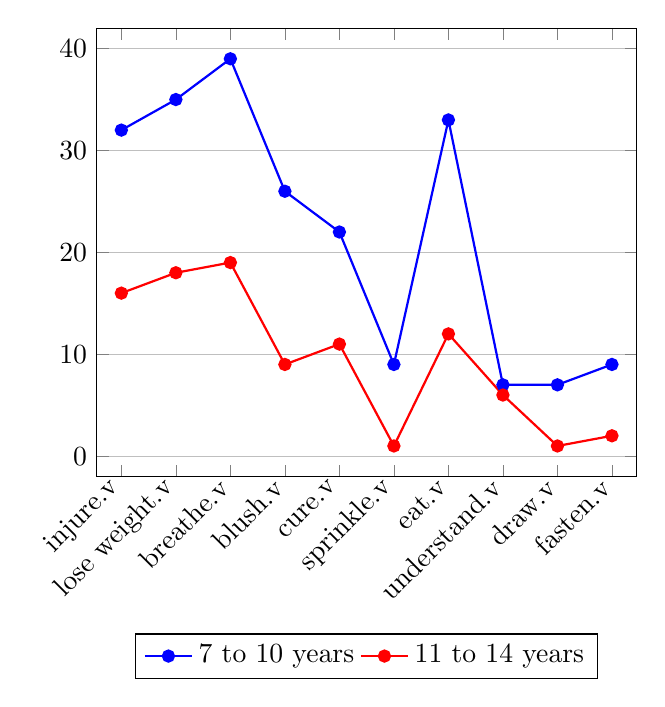
\begin{tikzpicture}
		\begin{axis}[
% 			ylabel={0,10,20,30,40},
			xtick=data,
			xticklabels={
				injure.v,
				lose weight.v,
				breathe.v,
				blush.v,
				cure.v,
				sprinkle.v,
				eat.v,
				understand.v,
				draw.v,
				fasten.v
			},
			x tick label style={rotate=45, anchor=east},
			legend style={at={(0.5,-0.35)}, anchor=north, legend columns=-1},
			ymin=0, ymax=40,
			ymajorgrids=true,
			enlargelimits=0.05
			]
			\addplot[
			color=blue,
			mark=*,
			thick
			]
			coordinates {
				(0,32)
				(1,35)
				(2,39)
				(3,26)
				(4,22)
				(5,9)
				(6,33)
				(7,7)
				(8,7)
				(9,9)
			};
			\addlegendentry{7 to 10 years}
			\addplot[
			color=red,
			mark=*,
			thick
			] coordinates {
				(0,16)
				(1,18)
				(2,19)
				(3,9)
				(4,11)
				(5,1)
				(6,12)
				(7,6)
				(8,1)
				(9,2)
			};
	\addlegendentry{11 to 14 years}
	\end{axis}
	\end{tikzpicture}
    \caption{Correlation score of verbs related to bodily functions and form}
    \label{fig:enter-label1}
\end{figure}

\begin{figure}
%     \includegraphics[width=\textwidth]{figures/Firgure 6.png}
\begin{tabularx}{0.7\textwidth}{XYY}
\lsptoprule
& 7 to 10 years & 11 to 14 years \\
\midrule
rain.v &     33 & 112 \\
blow.v &     33 & 110 \\
shine.v &    29 & 103 \\
sprinkle.v & 17 & 44) \\
thunder.v &  32 & 107 \\
blush up.v & 0  & 4   \\
jump.v &     1  & 6   \\
sleep.v &    1  & 6   \\
dream.v &    0  & 5   \\
wear.v &     1  & 6   \\
\midrule
\multicolumn{3}{l}{correlation score: 0.994704}\\
\lspbottomrule
\end{tabularx}

\vspace{\baselineskip}

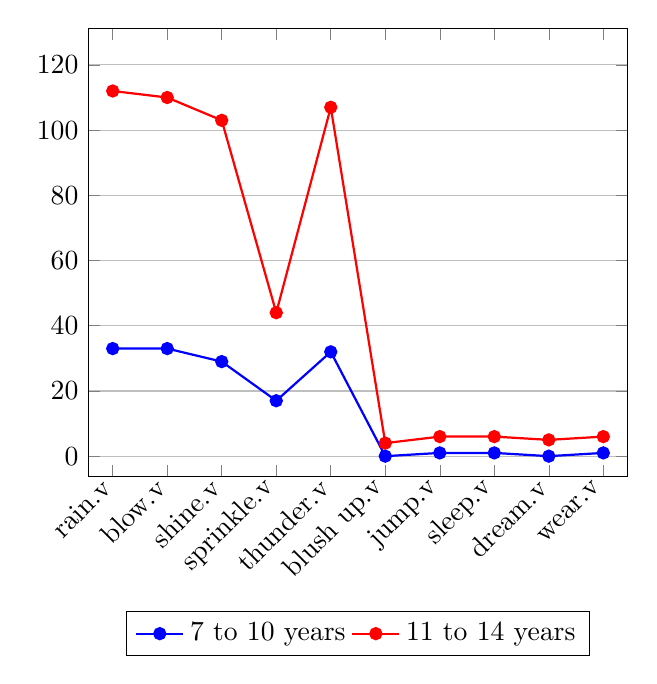
\begin{tikzpicture}
		\begin{axis}[
% 			ylabel={0,25,50,75,100,125},
			xtick=data,
			xticklabels={
				rain.v,
				blow.v,
				shine.v,
				sprinkle.v,
				thunder.v,
				blush up.v,
				jump.v,
				sleep.v,
				dream.v,
				wear.v
			},
			x tick label style={rotate=45, anchor=east},
			legend style={at={(0.5,-0.3)}, anchor=north, legend columns=-1},
			ymin=0, ymax=125,
			ymajorgrids=true,
			enlargelimits=0.05
			]
			\addplot[
			color=blue,
			mark=*,
			thick
			]
			coordinates {
				(0,33)
				(1,33)
				(2,29)
				(3,17)
				(4,32)
				(5,0)
				(6,1)
				(7,1)
				(8,0)
				(9,1)
			};
			\addlegendentry{7 to 10 years}
			\addplot[
			color=red,
			mark=*,
			thick
			] coordinates {
				(0,112)
				(1,110)
				(2,103)
				(3,44)
				(4,107)
				(5,4)
				(6,6)
				(7,6)
				(8,5)
				(9,6)
			};
	\addlegendentry{11 to 14 years}
		\end{axis}
	\end{tikzpicture}
    \caption{Correlation score of verbs of weather}
    \label{fig:enter-label2}
\end{figure}

\begin{figure}
%     \includegraphics[width=\textwidth]{figures/Firgure 7.png}
\begin{tabularx}{0.7\textwidth}{XYY}
\lsptoprule
& 7 to 10 years & 11 to 14 years \\
\midrule
drink.v,    & 21 & 62 \\
swallow.v,  & 20 & 57 \\
eat.v,      & 20 & 62 \\
chew.v,     & 20 & 63 \\
nibble.v,   & 20 & 51 \\
burn.v,     & 0 &  2 \\
wash.v,     & 1 &  1 \\
shave.v,    & 0 &  0 \\
beat.v,     & 1 &  1 \\
run.v       & 1 &  0 \\
\midrule
\multicolumn{3}{l}{correlation score: 0.993741} \\
\lspbottomrule
\end{tabularx}

\vspace{\baselineskip}

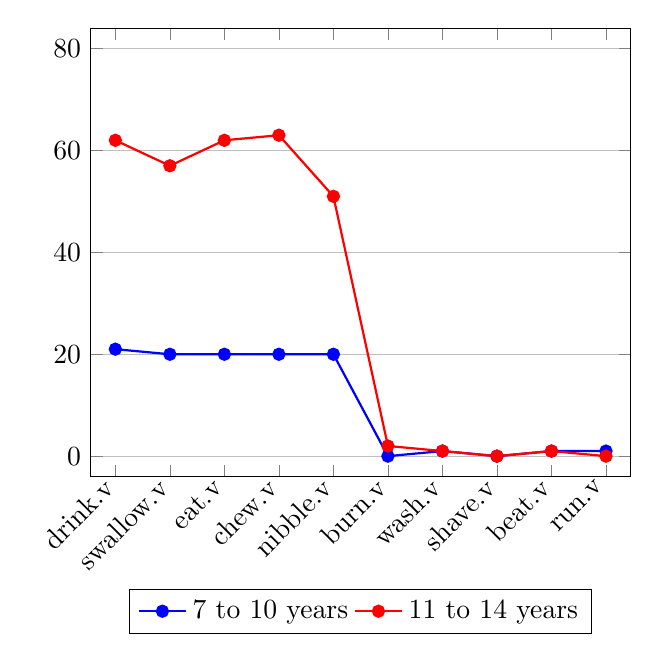
\begin{tikzpicture}
		\begin{axis}[
% 			ylabel={0,25,50,75,100,125},
			xtick=data,
			xticklabels={
				drink.v,
				swallow.v,
				eat.v,
				chew.v,
				nibble.v,
				burn.v,
				wash.v,
				shave.v,
				beat.v,
				run.v
			},
			x tick label style={rotate=45, anchor=east},
			legend style={at={(0.5,-0.25)}, anchor=north, legend columns=-1},
			ymin=0, ymax=80,
			ymajorgrids=true,
			enlargelimits=0.05
			]
			\addplot[
			color=blue,
			mark=*,
			thick
			]
			coordinates {
				(0,21)
				(1,20)
				(2,20)
				(3,20)
				(4,20)
				(5,0)
				(6,1)
				(7,0)
				(8,1)
				(9,1)
			};
			\addlegendentry{7 to 10 years}
			\addplot[
			color=red,
			mark=*,
			thick
			] coordinates {
				(0,62)
				(1,57)
				(2,62)
				(3,63)
				(4,51)
				(5,2)
				(6,1)
				(7,0)
				(8,1)
				(9,0)
			};
	\addlegendentry{11 to 14 years}
		\end{axis}
	\end{tikzpicture}
    \caption{Correlation score of verbs of consumption}
    \label{fig:enter-label3}
\end{figure}


The result for the three groups of verbs: verbs related to \editcolor{red}{bodily functions and form}, verbs of weather, and verbs of consumption, is  $R=0.943702806$, $R=0.994709117$, and $R=0.993740859$, respectively.

This is a strong positive correlation, which means that high X variable scores go with high Y variable scores (and vice versa).

This gives us reason to conclude that high selection values in a given group increase or at least confirm the values of the other group. If a verb has a high percentage ratio in 11- to 14-year-olds, the verb may be part of the basic vocabulary for that group, but also it will be part of the basic vocabulary of the 7- to 11-year-olds, and vice versa. In other words -- if a verb is mastered at the age of 7-10, then it is more likely to be part of a person's basic verb vocabulary at the age of 11-14. And vice versa -- if a verb is part of the basic verb vocabulary at the age of 11-14, it will be part of the basic verb vocabulary at a younger age.

On the other hand, the correlation between the frequency of use of the target verbs and the responses for each age group is different. The coefficient shows a moderate positive correlation between verb's frequency of use and responses of verb of weather, and also between verb's frequency of use and responses in the 11-14 age group of verbs related to \editcolor{red}{bodily functions and form}, \editcolor{red}{while in the other age group the correlation is defined as technically a positive one albeit weak}. \editcolor{red}{With verbs of consumption, the correlation also differs between the two age groups: the correlation in the 7-10 age group is technically a negative one, albeit weak, while the correlation in the age group 11-14 is again weak, but technically a positive one (see \tabref{fig:enter-label4}). Hence, the correlation between the frequency of use and the responses is not a significant factor in determining the dependence between the two variables.}

% \begin{figure}
%     \centering
%     \includegraphics[width=\textwidth]{figures/Firgure 4.png}
%     \caption{Correlation score between frequency and responses}
%     \label{fig:enter-label4}
% \end{figure}

\begin{table}
\caption{Correlation score between frequency and responses\label{fig:enter-label4}}
\begin{subtable}{\textwidth}
\centering
\begin{tabularx}{.9\textwidth}{XYYY}
\lsptoprule
verb.weather & frequency & 7--10 years & 11--14 years\\
\midrule
rain.v & 39.5 & 33 & 112 \\
shine.v & 22.29 & 29 & 103\\
blow.v & 10.49 & 33 & 110 \\
thunder.v & 3.96 & 32 & 107\\
sprinkle.v & 0.31 & 17 & 44\\
\midrule
\multicolumn{2}{l}{Correlation score}  & 0.51693 & 0.55848\\
\lspbottomrule
\end{tabularx}
\end{subtable}

\begin{subtable}{\textwidth}
\centering
\begin{tabularx}{.9\textwidth}{XYYY}
\lsptoprule
verb.body & frequency & 7--10 years & 11--14 years\\
\midrule
breathe.v & 51.61 & 39 & 19\\
cure.v & 24.66 & 22 & 11\\
injure.v & 22.1 & 32 & 16\\
lose weight.v & 8.18 & 35 & 18\\
blush.v & 4.38 & 26 & 9 \\
\midrule
\multicolumn{2}{l}{Correlation score}  & 0.48371 & 0.52761\\
\lspbottomrule
\end{tabularx}
\end{subtable}

\begin{subtable}{\textwidth}
\centering
\begin{tabularx}{.9\textwidth}{XYYY}
\lsptoprule
verb.consumption & frequency & 7--10 years & 11--14 years\\
\midrule
eat.v & 323.88 & 20 & 62\\
drink.v & 40.79 & 21 & 62\\
swallow.v & 7.44 & 20 & 57 \\
chew.v & 4.6 & 20 & 63\\
nibble.v & 2.12 & 20 & 51\\
\midrule
\multicolumn{2}{l}{Correlation score}  & -0.1401 & 0.38324\\
\lspbottomrule
\end{tabularx}
\end{subtable}
\end{table}

\subsection{Analysis of target verbs via associative stimuli}\label{subsect:4.2}

Word associations are among the key storage mechanisms in recall \citep{Glanzer1972}. Considering the intuitive nature of associations between the meaning of the verb, \editcolor{red}{the semantic frame it evokes and its frame elements}, we deem these types of tasks as the least difficult ones.

Association tasks are organised in two types. 

\subsubsection{Target verbs evoked by picture stimuli}

In the first type, four verbs are associated with a given picture, where at least one of the verbs refers to the main sense and is assumed to be part of the basic vocabulary, without additional encoding of the manner of action (which may be encoded by prefixes, suffixes, etc.). Results confirm that respondents prefer verbs from the core vocabulary, where the picture stimulus represents an element of the respective frames (mostly core frame elements, but non-core ones as well).

For example, the picture stimulus of a running man is most often associated by respondents with the verbs \textit{тичам} `run' (51.2\% among 7- to 10-year-olds; and 49.6\% among 11- to 14-year-olds) and \textit{бягам} `run' (39.5\% among 7- to 10-year-olds; and 44.7\% among 11- to 14-year-olds). Both verbs belong to the synset \{тичам; бягам\} -- \{run\}, verb.motion, with the definition `WN: move fast by using one's feet, with one foot off the ground at any given time’. The frame is \framename{Self\_\linebreak   Motion}; the picture stimulus \editcolor{red}{activates} the core frame element -- \fename{Self\_Mover}.

The picture stimulus of a shovel for the non-core frame element \fename{Instrument} is associated with the verb \textit{копая} `dig' in 70\% of responses, followed by \textit{рина} `shovel' in 19.2\%, while the prefixed verbs \textit{разривам} `dig up' and \textit{прекопавам} `dig up' are chosen by less than 10\% of the respondents. The picture stimulus of a bench for the core frame element \fename{Location} is associated with the verb \textit{седна} `sit', which may instantiate the frame \framename{Change\_posture} (it is preferred to the prefixed verbs \textit{поседна} `sit down' and \textit{приседна} `sit down' and the manner verb \textit{клекна} `squat').

The verb \textit{светя} `light, glisten' is associated with the picture stimulus of a light bulb, illustrating either both the \fename{Source} and \fename{Emission} core elements of the \framename{Emanating} frame, or the core elements of \fename{Figure} and \fename{Light} of the frame \framename{Location\_of\_light}. The verb is preferred over \textit{осветявам} `illuminate', \textit{светвам} `light up', \textit{блесвам} `shine'. 

Hesitancy among respondents, demonstrated by a more heterogeneous distribution of choices, is related to ambiguity or other possible association with the picture stimuli. For example, the picture stimulus of a dog standing upright on all fours is most often associated with the derivative \textit{изчаква} `await' (40\%) among 7- to 10-year-olds, less often with the non-derived verb \textit{чака} `wait' (24.4\%), followed by the manner verb \textit{дебна} `lurk' (17.8\%), while the 11- to 14-year-olds prefer the non-derivative \textit{чака} `wait' and \textit{дебне} `lurk' (both with 36\%), possibly due to the association of the dog with aggression (the verb \textit{дебна} `lurk' can be described by the frame \framename{Attack}). The picture corresponds to the \fename{Protagonist} core element of the \framename{Waiting} frame. 

Among all the tasks, clear preference (by over 50\% of the respondents with clear margin with respect to the other possible choices) is given to basic (mostly non-derived) verbs referring to a simple action without additional specification of the manner of action, namely: \textit{тичам} `run', \textit{бягам} `run'; \textit{копая} `dig' (\textit{рина} `shovel', \textit{светя} `shine' (\textit{осветявам} `shine on', \textit{прегръщам се} `hug' (\textit{гуш\-кам се} `cuddle', \textit{седна} `sit' (\textit{поседна} `sit', \textit{подстриже} `cut (hair)' (\textit{оформя} `form', \textit{подрежа} `cut', \textit{налея} `pour', \textit{сипя} `pour', \textit{горя} `burn' (\textit{изгарям} `burn out'. 

\subsubsubsection{Correlation scores of the experiment results}

The correlation scores between the best and the second best answer (in \%) are negative (as the children systematically have given a single answer) and statistically significant (Spearman’s rho coefficient of the answers of 7- to 10-year-olds is $r_s = -0.74772$, and of the answers of 10- to 14-year-olds is $r_s = -0.82805$). The correlation scores between the best answers of the two age groups show strong positive correlation and are statistically significant ($r_s =0.84242$) -- see \figref{fig:enter-label5}.

\begin{figure}
%     \includegraphics[width=\textwidth]{figures/Fig5.png}
\begin{tabularx}{0.7\textwidth}{XYY}
\lsptoprule
Preferred verb & 7 to 10 years (\%) & 11 to 14 years (\%) \\
\midrule
  hear.v  & 73.8 & 79.3)\\
  light.v  & 73.2 & 69)\\
  dig.v  & 62.2 & 71.9)\\
  embrace.v  & 82.9 & 86.8)\\
  run.v  & 51.2 & 49.6)\\
  burn.v  & 68.3 & 68.3)\\
  await.v  & 24.4 & 36)\\
  sit.v  & 80   & 61.5)\\
  cut hair.v  & 53.6 & 54.8)\\
  fill.v & 44.4 & 44.6 \\
  \midrule
  \multicolumn{3}{l}{Correlation score: 0.887412 (strong positive),}\\
  \multicolumn{3}{l}{$r_s$ = 0.84242, $p$ (2-tailed) = 0.00222} \\
  \lspbottomrule
\end{tabularx}

\vspace{\baselineskip}

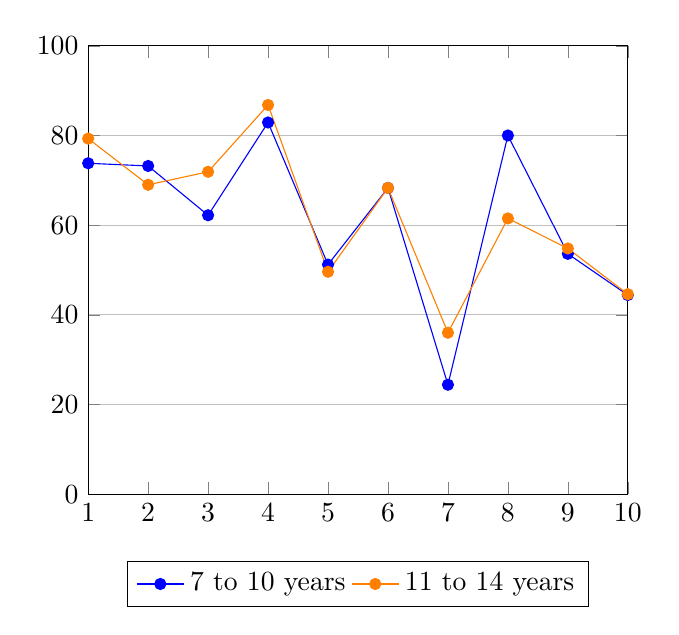
\begin{tikzpicture}
		\begin{axis}[
			xmin=1, xmax=10,
			ymin=0, ymax=100,
			xtick={1,2,...,10},
			ytick={0,20,...,100},
			ymajorgrids=true,
			legend style={at={(0.5,-0.15)}, anchor=north, legend columns=2}
			]
			\addplot[color=blue,mark=*] coordinates {
				(1,73.8)
				(2,73.2)
				(3,62.2)
				(4,82.9)
				(5,51.2)
				(6,68.3)
				(7,24.4)
				(8,80)
				(9,53.6)
				(10,44.4)
			};
			\addlegendentry{7 to 10 years}
			\addplot[color=orange,mark=*] coordinates {
				(1,79.3)
				(2,69)
				(3,71.9)
				(4,86.8)
				(5,49.6)
				(6,68.3)
				(7,36)
				(8,61.5)
				(9,54.8)
				(10,44.6)
			};
			\addlegendentry{11 to 14 years}
		\end{axis}
	\end{tikzpicture}
    \caption{Correlation score between best answers of the two age groups(\editcolor{blue}{blue line -- 7- to 10-year-olds; orange line -- 10- to 14-year-olds).}}
    \label{fig:enter-label5}
\end{figure}

\subsubsection{Target verbs evoked by situation stimuli}

In thе second type of tasks, the picture stimulus also represents \editcolor{red}{a possible realisation of a core frame element} but respondents have to choose among ten verbs from different synsets, which may be \editcolor{red}{analysed} by different semantic frames. Five of the ten verbs are expected to be chosen, three are completely inappropriate, while the rest two are appropriate to a certain degree. 

For example, the picture stimulus showing objects related to eating and drinking is associated with the verbs \textit{закусвам} `to eat breakfast' (20.9\%\footnote{All answers are equal to 100 percent, and the ratio is calculated accordingly.}  among 7- to 10-year-olds; and 21.9\% among 11- to 14-year-olds), \textit{хапвам} `snack' (17.4\% and 16.7\%, respectively), \textit{ям} `eat' (17.4\% and 16\%, respectively), \textit{похапвам} `snack' (15.1\% and 16\%, respectively), and \textit{пия} `drink' (15.1\% and 15\%, respectively). All five verbs may be \editcolor{red}{analysed} by the frame \framename{Ingestion}, with the picture stimulus corresponding to the core frame element \fename{Ingestibles}. The preference for the manner verb \textit{закусвам} `eat breakfast' may be related to the time constraint in the sentence stimulus (\textit{Сутрин} `in the morning' which illustrates the non-core frame element \fename{Time}). The picture stimulus -- arranged objects related to food -- also determines the next most frequent choices -- \textit{готвя} `cook' (4.7\% and 8.2\%, respectively) and \textit{подреждам} `arrange' (3.5\% and 3.9\%, respectively). 

Here, the disagreement among the focus groups is much lower probably due to the larger set of possible answers. The correlation scores between the highest probable and the highest less probable answer show weak positive correlation, but are not statistically significant (Spearman’s rho coefficient of the answers of 7- to 10-year-olds is $r_s = -0.74772$, and of the answers of 10- to 14-year-olds is $r_s = -0.82805$). 

\subsubsubsection{Correlation scores of the experiment results}

The correlation scores between the average of the target answers between the two age groups again show strong positive correlation and are statistically significant ($r_s =0.81818$) -- see \figref{fig:enter-label6}.

\begin{figure}
%     \includegraphics[width=\textwidth]{figures/Fig6.png}
\begin{tabularx}{0.7\textwidth}{XYY}
\lsptoprule
\multicolumn{3}{c}{Average of the target verbs}\\
\midrule
Subtask & 7 to 10 years (\%) & 11 to 14 years (\%) \\
 \midrule
 1 & 17.68  &   17.68  \\
 2 & 15.94  &   15.94  \\
 3 & 16.66  &   17.56  \\
 4 & 16.14  &   16     \\
 5 & 17     &   17.64  \\
 6 & 18     &   17.64  \\
 7 & 13.86  &   13.06  \\
 8 & 18.22  &   17.36  \\
 9 & 18.42  &   18.26  \\
 10 & 17.18 &   17     \\
 \midrule
  \multicolumn{3}{l}{Correlation score: 0.937487 (strong positive)} \\
  \multicolumn{3}{l}{$r_s$ = 0.81818, $p$ (2-tailed) = 0.00381} \\
\lspbottomrule
\end{tabularx}

\vspace{\baselineskip}

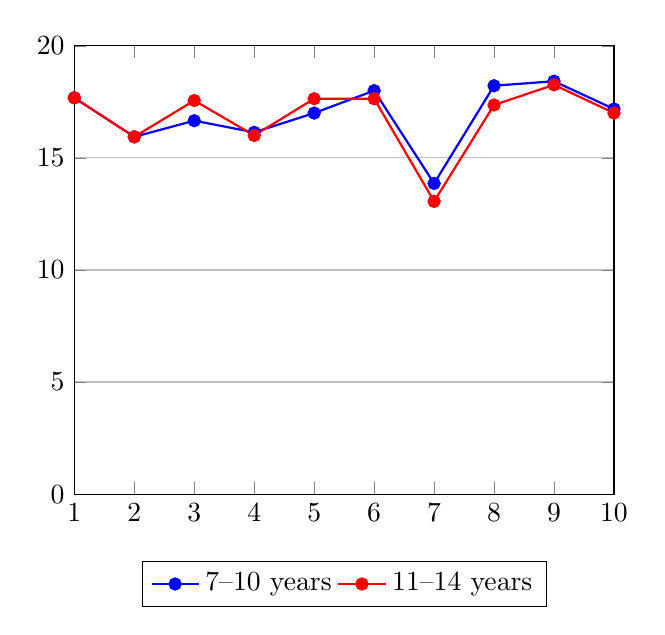
\begin{tikzpicture}
		\begin{axis}[
			xlabel={},
			ymajorgrids=true,
			ytick={0,5,10,15,20},
			xtick = {1,2,...,10},
			ymin = 0,
			ymax = 20,
			xmin = 1,
			xmax = 10,
			legend style={at={(0.5,-0.15)}, anchor=north, legend columns=2}
			]
			\addplot[
			color=blue,
			mark=*,
			thick
			]
			coordinates {
				(1,17.68)
				(2,15.94)
				(3,16.66)
				(4,16.14)
				(5,17)
				(6,18)
				(7,13.86)
				(8,18.22)
				(9,18.42)
				(10,17.18)
			};
			\addplot[
			color=red,
			mark=*,
			thick
			] coordinates {
				 (1,17.68)
				 (2,15.94)
				 (3,17.56)
				 (4,16)
				 (5,17.64)
				 (6,17.64)
				 (7,13.06)
				 (8,17.36)
				 (9,18.26)
				 (10,17)
			};
			\legend{7--10 years, 11--14 years};
		\end{axis}
	\end{tikzpicture}
    \caption{Correlation score between the recognised target verbs between the two age groups(\editcolor{blue}{blue line -- 7- to 10-year-olds; orange line -- 10- to 14-year-olds).}}
    \label{fig:enter-label6}
\end{figure}

This basically confirms the conclusion from the thematically related tasks that there is correlation between basic verbs acquired by the two age groups. However, verbs' senses do not associate with each other. 

Most of the verbs in both tasks \editcolor{red}{evoke semantic frames} that are linked to the \framename{Event} top frame, as follows. 

The frame \framename{Motion} is linked via inheritance to \framename{Self\_motion}, \framename{Motion\_noise}, and \framename{Motion\_scenario} via usage to \framename{Departing}, \framename{Bringing}, \framename{Removing}, \framename{Emanating}, and via subframe to \framename{Halt}. 

The frame \framename{Intentionally\_affect} is linked to \framename{Cutting}, \framename{Education\_teaching}, \framename{Arranging}, \framename{Grooming}, as well as to \framename{Communication}, which, in its turn, is linked via inheritance to \framename{Communication\_manner} and \framename{Communication\_noise} and via usage to \framename{Questioning}. 

The frame \framename{Intentionally\_create} is linked to \framename{Cooking\_creation}, \framename{Create\_physical\_artwork}, which is linked to \framename{Create\_representation}.

The frame \framename{Intentionally\_act} is linked to \framename{Change\_posture}, \framename{Perception\_active}, and \framename{Manipulation}, which is further linked via inheritance to \framename{Ingestion}. 

The picture stimuli most often activate core frame elements such as: [\fename{Agent} | \fename{Communicator} | \fename{Speaker} | \fename{Teacher} | \fename{Creator} | \fename{Protagonist} | \fename{Self\_\linebreak mover} (Sentient)] (where [\fename{Protagonist} and \fename{Self\_mover} can also be represen\-ted by an animal); [\fename{Theme} | \fename{Vehicle} (Physical object)], as well as \fename{Goal}, \fename{Body\_part}, \fename{Patient}, \fename{Source}, \fename{Ingestibles}, \fename{Medium}, \fename{Message}. The non-core frame elements include: \fename{Instrument}, \fename{Means}, as well as \fename{Source}, \fename{Goal}, \fename{Body\_part}. 

The most frequent non-core frame element, \editcolor{red}{evoked} by the picture stimuli, is \fename{Instrument}, while the most frequent core frame element is \fename{Theme}. The picture stimulus may activate the preference to one verb with a core frame element instead of another with a non-core frame element -- for example, a picture of an ear is most often associated with the verb \textit{чувам} `hear' (74\% and 79.3\% in the two focus groups, respectively), which may be \editcolor{red}{analysed} by the frame \framename{Perception\_experience} with the core frame element \fename{Body\_part}; and less often with the verb \textit{слушам} `listen', which may be \editcolor{red}{analysed} by the frame \framename{Perception\_active} where the \fename{Body\_part} frame element is non-core (and unexpressed).

Hesitancy among respondents -- demonstrated when a verb is chosen by a number of respondents below the mean -- is observed if the picture stimulus does not entirely meet the characteristics of the frame element. For example, the picture of the dog standing, mentioned above, is associated with the verbs \textit{чака} `wait' by 36\% among the 11- to 14-year-olds (but by 24.40\% among the 11- to 14-year-olds, which is below the mean), while for the prefixed verb \textit{изчаква} `wait' the ratio is 37.80\% among the 7- to 10-year-olds against only 8\% of the 11- to 14-year-olds, while the preference to \textit{дебне} `lurk' is the opposite -- 17.80\% among the 7- to 10-year-olds (which is below the mean) and 36\% among the 11- to 14-year-olds. The frame element \fename{Protagonist} is specified as (Sentient), while the picture is of an animal. This is also the only task of the ten from the first type with such heterogeneous preference patterns (in five tasks, the preference is given to only one of the verbs; in two -- to two verbs, while in the rest the two focus groups are unanimous about one verb, but do not agree on the second possible choice). 


\begin{table}
\begin{tabularx}{\textwidth}{p{2.1cm}llp{1.8cm}X%p{1.4cm}
}
\lsptoprule
Verb & 7-10 yrs& 11-14 yrs& Frame & Frame elements %&Activated
\\
\midrule
\textit{плава} \newline `sail' & 22.7\% & 20.3\% & \framename{Motion} & \fename{Area}; \fename{Direction}; \fename{Distance}; \fename{Goal}; \fename{Path}; \fename{Source}; \underline{\fename{Theme}} (PhysObj) %& \fename{Theme}
\\
\midrule
\textit{плува} \newline `swim' & 8\% & 7.5\% & \framename{Self\_\linebreak motion} & \fename{Area}; \fename{Direction}; \fename{Goal}; \fename{Path}; \fename{Self\_\linebreak mover} (Sent); \fename{Source} %&  \textit{-} 
\\
\midrule
\textit{акостира} \newline `shore' & 12.5\% & 11.4\% & \framename{Vehicle\_\linebreak  landing} & \fename{Goal}; \underline{\fename{Vehicle}} %(PhysObj)% & \fename{Vehicle}  
\\
\midrule
\textit{потегля} \newline`depart' & 17\% & 18.3\% & \framename{Departing} & \fename{Source} (Loc); \underline{\fename{Theme}} %(PhysObj) %& \fename{Theme}  
\\
\midrule
\textit{спира}  \newline `halt' & 9.1\% & 7.8\% & \framename{Halt} & \fename{Theme} %(Physical object) %& \textit{-} 
\\
\midrule
\textit{превозва} \newline `carry' & 19.3\% & 19.9\% & \framename{Bringing} & \fename{Agent} (Sent); \fename{Area}; \underline{\fename{Carrier}}; \fename{Goal}; \fename{Path}; \fename{Source}; \fename{Theme} %(PhysObj) %& \fename{Carrier}  
\\ 
\midrule
\textit{износва} \newline `carry off' & 6.8\% & 5.9\% & \framename{Bringing} & \fename{Agent} (Sent); \fename{Area}; \underline{\fename{Carrier}}; \fename{Goal}; \fename{Path}; \fename{Source}; \fename{Theme} %(PhysObj) %& \fename{Carrier} 
\\ 
\midrule
\textit{продължава} \newline `keep on' & 4.5\% & 7.25\% & \framename{Activity}\_{}\linebreak \framename{ongoing} & \fename{Agent} (Sent); \fename{Activity}; \fename{Duration} %& N/A  
\\ 
\midrule
\textit{писука} \newline `chirp' & 0\% & 0.7\% & N/A & N/A %& N/A  
\\
\midrule
\textit{мълчи} \newline `be quiet' & 0\% & 1\% & N/A & N/A %& N/A  
\\
\lspbottomrule
\end{tabularx}
\caption{Results of Association task -- a picture of a ship (Activated frame element is underlined)}
\label{tab:chapterhandle:keytotable5}
\end{table}

\tabref{tab:chapterhandle:keytotable5} illustrates the distribution of the respondents' choices in one of the tasks where the verbs may activate different semantic frames. The respondents have associated the meaning of the verbs \editcolor{red}{stimulated by the meaning of a core frame element} -- for example, the verb \textit{плува} `swim' is \editcolor{red}{analysed} more often by the frame \framename{Self\_motion} and sentient \fename{Agent} instead of  the semantic frame \fename{Motion} and \fename{Theme} frame elements.

\subsubsection{Prevailing semantic frame preferences in the respondents' selection}\label{subsect:4.2.1}

\editcolor{blue}{The results of the experiment on evoking verbs via associative stimuli allow us to} summarise the most frequently selected  frames of the experiment  target verbs. The description of the frame includes a list of Bulgarian verbs, their semantic frame definition, their frame elements, information for the selectional specifics, and syntactic representation of the frame elements. 
\newpage

\begin{enumerate}
\item
\begin{description}[font=\normalfont]
\item[Semantic Frame:] \framename{Cutting}
\item[Target verbs:] \textit{кълцам} `chop'; \textit{режа} `cut’ (\textit{изрязвам, отрязвам, наряз\-вам, разрязвам} are language-specific verbs derived from the verb \textit{режа} `cut')
\item[Frame Definition:] `An \fename{Agent} cuts an \fename{Item} into \fename{Pieces} using an \fename{Instrument} (which may or may not be expressed).’
\item[Frame Elements:] \fename{Agent} // \fename{Item} // \fename{Pieces}
\item[Semantic and selectional specifics:] NP \fename{Agent} \{person\} \textit{cut}.v NP \fename{Item} \{artifact\}, PP \fename{Pieces} \{piece\}
\end{description}

\item 
\begin{description}[font=\normalfont]
\item[Semantic Frame:] \framename{Ingestion}
\item[Target verbs:] \textit{ям}~ `eat',~ \textit{похапвам}~ `snack',~ \textit{хапвам}~ `eat',~ \textit{закусвам} `have breakfast', \textit{гълтам} `swallow', \textit{гриза} `nibble', \textit{пия} `drink'
\item[Frame Definition:] `An \fename{Ingestor} consumes food or drink \fename{Ingestibles}, and this entails putting the \fename{Ingestibles} in the mouth for delivery to the digestive system.'
\item[Frame Elements:] \fename{Ingestor} // \fename{Ingestibles} 
\item[Semantic and selectional specifics:] NP \fename{Ingestor} \{person\} | \{animal\} \textit{eat}.v NP \fename{Ingestibles} \{food\} | \{nutrient\} | \{meat\} | \{fish\} | \{vegetable\} | \{fruit\}

     or
     
     NP \fename{Ingestor} \{person\} | \{animal\} \textit{drink}.v NP \fename{Ingestibles} \{beverage\} | \{alcoholic drink\} | \{water\}
\end{description}
     

\item 
\begin{description}[font=\normalfont]
\item[Semantic Frame:] \framename{Make\_noise}
\item[Target verbs:] \textit{свиря} `play', \textit{викам} `shout', \textit{крещи} `scream', \textit{писука} `chirp', \textit{тананикам} `hum'
\item[Frame Definition:] `A physical entity, construed as a point -- \fename{Sound}\_\linebreak \fename{source}, emits a \fename{Sound}. This includes animals and people making noise with their vocal tracts.'
\item[Frame Elements:] \fename{Sound} // \fename{Sound\_source} // \fename{Noisy\_event}
\item[Semantic and selectional specifics:]  \textit{chirp}.v NP \fename{Sound} \{sound\}, PP \fename{Sound}\_\linebreak \fename{source} \{mouth\}, PP \fename{Noisy\_event} \{occurrence\} 
\end{description}

\newpage
\item
\begin{description}[font=\normalfont]
\item[Semantic Frame:] \framename{Motion}
\item[Target verbs:] \textit{пътува} `travel', \textit{лети} `fly', \textit{духа} `blow', \textit{плава} `float', \textit{плува} `drift' (English verbs for \textit{плава} `sail' and \textit{плува} `swim' are recognised as \framename{Self\_Motion} verbs in FrameNet.)
\item[Frame Definition:] `Some entity \fename{Theme} starts out in one place (Source) and ends up in some other place \fename{Goal}, having covered some space between the two \fename{Path}. Alternatively, the \fename{Area} or \fename{Direction} in which the \fename{Theme} moves or the \fename{Distance} of the movement may be mentioned.' 
\item[Frame Elements:] \fename{Area} // \fename{Direction} // \fename{Distance} // \fename{Theme}  // \fename{Source} // \fename{Goal} // \fename{Path}
\item[Semantic and selectional specifics:] PP \fename{Area}, \fename{Direction}, \fename{Distance}, \fename{Path}, \fename{Source}, \fename{Goal} can be in some case or another -- \{location\} | \{path\} | \{way\} | \{longness\} | \{land\} | \{area\}, NP [\fename{Theme}] \{physical object1\} 
\end{description}

\item 
\begin{description}[font=\normalfont]
\item[Semantic Frame:] \framename{Self\_motion}
\item[Target verbs:] \textit{бягам} `run', \textit{тичам} `run', \textit{скачам} `jump', \textit{подскачам} `jump', \textit{подрипвам} `caper'
\item[Frame Definition:] `The \fename{Self\_mover}, a living being, moves under its own direction along a \fename{Path}. Alternatively or in addition to \fename{Path}, an \fename{Area}, \fename{Direction}, \fename{Source}, or \fename{Goal} for the movement may be mentioned.'
\item[Frame Elements:] \fename{Area}; \fename{Direction}; \fename{Goal}; \fename{Path}; \fename{Self mover}; \fename{Source}
\item[Semantic and selectional specifics:] NP \ \fename{Self\_mover} \{person\} \  \textit{run}.v \ PP \fename{Area}, \fename{Direction}, \fename{Goal}, [\fename{Path}], \fename{Source} can be in some case or another -- \{location\} | \{path\} | \{way\} | \{land\} | \{area\}
\end{description}
\end{enumerate}

\subsection{Analysis of contextually related verbs}\label{subsect:4.3}

The contextual competency of respondents was tested in two types of tasks with different level of difficulty -- sentence usage of thematically related verbs and textual usage of verbs. The results of the two approaches are split. Respondents were able to handle thematically related verbs placed in a specific sentence context, but showed considerable difficulty in selecting verbs in a connected text.   

\subsubsection{Target verbs in a sentence context}\label{subsubsect:4.3.1}

The selected target verbs and the corresponding sentences denote situations and actions in respondents' everyday life. The results of the experiment showed that over 90\% of the participants recognised the meaning of the verbs and use them correctly in the context.  \editcolor{blue}{In this type of tasks we use the syntactic realisation of core frame elements of a semantic frame into the sentences as stimuli for the selection of target verbs.}  The sentences illustrating the verb's context represent situations evoked by semantic frames. \editcolor{red}{The illustrative sentence for the verb \textit{ям} `eat' is analysed by the semantic frame \framename{Ingestion}, \textit{поръся} `sprinkle' is analysed by the semantic frame \framename{Filling}, \textit{налея} `pour' is analysed by the frame \framename{Container\_\linebreak focused\_placing}. 

All sentences have core frame element Agent in the subject position with a null instantiation. The other core frame elements  are: \fename{Ingestibles} (\textit{delicious and healthy food}); \fename{Theme} (\textit{sprinkle salt}) \fename{Goal}  (\textit{on the toast}); \fename{Theme} (\textit{juice}); \fename{Goal} (\textit{into a large glass}).} 

\editcolor{red}{In other sentences, however, the frames \framename{Absorb\_\linebreak heat} \textit{сваря} `boil', \framename{Apply\_heat} \textit{препека} `toast', \framename{Grinding} \textit{настържа} `grate' remain with null instantiations of the frame elements. For example, in the sentence \textit{I boiled an egg} the \fename{Heat\_source} is not evoked, while in the sientence \textit{Gonna grate some cheese}, the  core frame  element \fename{Static\_object} or \fename{Topic} -- the surfaces that rub against each other -- \textit{ренде} `grater' is not instantiated. However, there are enough elements that are explicit, including for non-core frame elements, e.g., \textit{I squeeze oranges for my favourite juice} [\fename{Goal}] or \textit{I will drink with relish} [\fename{Manner}].}

In the examples below we demonstrate the application of semantic-syntactic frames as stimuli in the concrete sentences from the tasks: 


\begin{exe}  
\ex \label{bg:diff-vb1a} \textit{Сутрин обичам да} [pro]$_{ \feinsub{Ing}}$ \textit{\textbf{ЯМ}} [\framename{Ingestion}] [\textit{вкусна и здравословна\linebreak храна}]$_{\feinsub{Ingbles}}$.  \\[-0.8em]
\glt `In the morning I like to eat delicious and healthy food.'

\ex \label{bg:diff-vb1b} \textit{Ето сега} [pro]$_{\feinsub{Age}}$ \textbf{\textit{\uppercase{изцеждам}}} [\framename{Manipulation}] [\textit{портокали}]$_{\feinsub{Ent}}$ [\textit{за лю\-бимия сок}]$_{\feinsub{Result}\  (non-core)}$.\\[-0.8em]
\glt `Right now I am squeezing oranges for my favorite juice.' \\
* Unexpressed frame elements [\fename{Bodypart\_of\_agent}] -- the part of the \fename{Agent}'s body being used to manipulate the \fename{Entity}.
 
\ex \label{bg:diff-vb1c}  \textit{Преди това} [pro]$_{\feinsub{Age}}$ \textit{\textbf{\uppercase{сварих}}} [\framename{Absorb\_heat}] [\textit{едно яйце}]$_{\feinsub{Ent}}$ [\textit{в тен\-джера}]$_{\feinsub{Container}}$. \\[-0.8em]
\glt `Previously, I boiled  an egg  in a pot.' \\
* The source of heat treatment [\fename{Heat\_source}] is not expressed.

\ex \label{bg:diff-vb1d} \textit{В момента} [pro]$_{\feinsub{Age}}$ \textit{\textbf{\uppercase{режа}}} [\framename{Cutting}] [\textit{домата}]$_{\feinsub{Item}}$ [\textit{на парчета}]$_{\feinsub{Pieces}}$.  \\[-0.8em]
\glt `Currently, I am slicing the tomato into pieces.'
  
\ex \label{bg:diff-vb1e} \textit{Взех}  \textit{филийки хляб}, \textit{за да} [\textit{ги}]$_{\feinsub{Food}}$ [pro]$_{\feinsub{Cook}}$\textit{\textbf{\uppercase{препека}}} [\framename{Apply\_heat}] [\textit{в тостера}]$_{\feinsub{HeatIns}}$. \\[-0.8em]
\glt `I  took slices of bread to toast them in the toaster.' \\
* Null instantiation frame elements are: [\fename{Container}] -- the object where food is stored and to which heat is applied, [\fename{Heating\_instrument}] -- the object that emits heat, [\fename{Temperature\_setting}] -- the temperature at which the food is processed.

\ex \label{bg:diff-vb1f} \textit{Когато} \textit{филийките} \textit{са готови}, [pro]$_{\feinsub{Age}}$ \textit{ще} [\textit{ги}]$_{\feinsub{Goal}}$ \textit{\textbf{\uppercase{намажа}}} [\framename{Fil\-ling}] [\textit{с масло}]$_{\feinsub{Thm}\  (PhysObj)}$.\\[-0.8em]
\glt `When the slices are ready, I will butter them.'

\ex \label{bg:diff-vb1m} \textit{След това} [pro]$_{\feinsub{Age}}$ \textit{ще} \textit{\textbf{\uppercase{поръся}}} [\framename{Filling}] [\textit{сол}]$_{\feinsub{Thm}\ (PhysObj)}$ [\textit{върху фи\-лийката}]$_{\feinsub{Goal}}$.\\[-0.8em]  
\glt `Then I  will sprinkle salt on the slice.'

\ex \label{bg:diff-vb1g}  [\textit{Върху филийката}]$_{\feinsub{Place}\ (non-core)}$ \textit{ще} \textit{\textbf{\uppercase{настържа}}} [\framename{Grinding}] \textit{и} [\textit{малко кашкавал}]$_{\feinsub{Pat}}$.\\[-0.8em]
\glt `On top of the slice, I will grate some cheese.'
  
    \ex \label{bg:diff-vb1h} \textit{Накрая} [pro]$_{\feinsub{Age}}$ \textit{ще} \textit{\textbf{\uppercase{налея}}} [\framename{Container\_focused\_placing}] [\textit{портокалов сок}]$_{\feinsub{Thm}\ (PhysObj)}$ [\textit{в голяма чаша}]$_{\feinsub{Goal}}$...\\[-0.8em]
\glt `Finally I will pour orange juice into a large glass...'

\ex ... \textit{и} [pro]$_{\feinsub{Ing}}$ \textit{ще} \textit{\textbf{\uppercase{изпия}}} [\framename{Ingestion}] [\textit{с наслада}]$_{\feinsub{Manner}\ (non-core)}$ [\textit{вкус\-ната напитка}]$_{\feinsub{Ingbles}}$.\\[-0.8em]
\glt `... and I  will drink  with delight the delicious drink.'
\end{exe}


\subsubsection{Target verbs in a text}\label{subsubsect:4.3.2}

The tasks aimed at textual usage of words gather information about the respondents' ability to acquire knowledge and to research, evaluate, and control this knowledge. Thus, they are the most difficult ones and combine a complex of stimuli. The tasks imply that the participants have to take into account the lexical, grammatical, and morpho-semantic specificity of the verbs studied within a task (verbs with concrete and abstract meanings from all semantic classes, i.e., cognitive verbs, verbs of emotions, stative verbs, motion verbs, etc.).

Verbs that do not fit the specific usage in the text are also embedded in the sentences. They are selected on the following principle -- a phonological competitor (a paronym) of the correct verb see (Examples \ref{bg:diff-vb1}d, \ref{bg:diff-vb2}b); a verb similar in meaning, but with a syntactic realisation incompatible with the context (Examples \ref{bg:diff-vb2}b, \ref{bg:diff-vb3}a) or which does not meet the lexico-grammatical requirements for the verb form -- transitivity, reflexiveness etc. (Example \ref{bg:diff-vb2}c, \ref{bg:diff-vb3}c). These principles are illustrated in the short text part -- adapted fragment of ``Alice in Wonderland'' used in one of the tasks.

\largerpage
\begin{exe}  
\ex \label{bg:diff-vb1}
\textit{Алиса \textbf{\uppercase{скучаеше}}} (страдаше (a), доскучаваше (b), нуждаеше (c)) \textit{и си \textbf{\uppercase{мислеше}}} (приспиваше (d), успиваше (e), колебаеше (f)) \textit{дали да \textbf{\uppercase{набере}}} (прибере (g), отнесе (h), обере (i)) \textit{един букет от маргаритки в тежката следобедна горещина.}\\[-0.8em]
\glt `Alice was beginning to get very bored (suffer (a), beginning to suffer (b), need (c))\footnote{The translation of the alternative verbs in the tasks is literal and does not follow the above mentioned criteria -- paronym, synonym, etc.} and she was \textbf{considering} (dozing off (d), starting to sleep (e), hesitating (f)) in her own mind whether \textbf{to pick} (take (g), bring (h), steal (i)) a branch of daisies in the hot afternoon.' 
   
\ex \label{bg:diff-vb2}
\textit{През това време един Бял Заек със светлочервени очи} \textit{\textbf{\uppercase{подскочи}}} (посочи (a), поклати (b), изсмя (c)) \textit{край нея.} 
\\[-0.8em]
\glt `At the same time a White Rabbit with pink eyes \textbf{ran} (pointed (a), shook (b), laughed (c)) close by her.'
   
\ex \label{bg:diff-vb3}
\textit{Това не се} \textit{\textbf{\uppercase{стори}}} (оказа (a), престори (b), помисли (c)) \textit{необикновено на Алиса и тя не} \textit{\textbf{\uppercase{се изненада}}} (изстрада (d), измисли (e), сметна(f) \textit{дори когато} \textit{\textbf{\uppercase{чу}}} (слуша (g), попита (h), нахлу (i)) \textit{как Заекът} \textit{\textbf{\uppercase{си гово\-ри}}} (въобразява (a), внушава (b), спори (c)) \textit{„О, божичко, божичко!“}. 
\\[-0.8em]
\glt `There \textbf{was} (did (a), pretended (b), thought (c)) nothing so very \textbf{remarkable} in that; nor \textbf{did} Alice \textbf{think} (suffer (d), invent (e), count (f) it so very much out of the way to \textbf{hear} (listen (g), ask (h), invade (i)) the Rabbit \textbf{say} (imagine (a), suggest (b), argue (c)) to itself, ``Oh dear! Oh dear!'''
 
\ex \label{bg:diff-vb4}
\textit{По-късно, като} \textit{\textbf{\uppercase{размисли}}} (замисли (a), измисли (b), сметна (c)), \textit{\textbf{\uppercase{реши}}} (разреши (d), представи (e), каза (f)), \textit{че това е доста необичай\-но}. 
\\[-0.8em]
\glt `When she \textbf{thought} (considered (a), imagined (b), reckoned (c)) it over afterwards, it \textbf{occurred} (allowed (d), presented (e), said (f)) to her that she ought to have wondered at this.'\footnote{The original Bulgarian translation of the text is adapted and simplified.}
\end{exe}

In addition, the task \editcolor{blue}{relies on respondents' knowledge of semantic and causa\-tive relations between sequences of verbs and uses those contextual relations as stimuli:}
\begin{itemize}
\item \editcolor{blue}{semantic relation between target verbs as a contextual stimuli. For example: \textit{скучаеше и си мислеше} (was bored and thought about); \textit{размисли} (thought) $\longrightarrow$ \textit{реши} (decided) in Example \ref{bg:diff-vb4};
\item grammatical selection of a target verbs in the main clause and the target verb in the subordinate clause as contextual stimuli \textit{скучаеше и си мислеше} (was bored and thought about) $\longrightarrow$ \textit{дали да набере} (whether to pick) in Example \ref{bg:diff-vb1}; \textit{чу} (heard) $\longrightarrow$ \textit{как си говори} (her talk) in Example \ref{bg:diff-vb2};
\item grammatical combinability between target verbs prepositions and conjunctions (Examples \ref{bg:diff-vb2}, \ref{bg:diff-vb3}).}\\
\end{itemize}

Another criterion of difficulty is the need of consideration of the information in the whole context used as last level stimuli of selection. All verb choices are presented shuffled below the text. Although in some sentences an alternative choice is possible (for example, Алиса мислеше и си каза дали да посочи... (Alice thought and said to herself whether she should indicate...) in composing the overall text, the alternatives are not acceptable.

\begin{table}
\begin{tabularx}{\textwidth}{p{1.6cm} p{1.7cm} ll X %p{3.2cm}
}
\lsptoprule
Verb & Semantic class & 7-10 yrs & 11-14 yrs & Frame %& Context
\\
\midrule
\textit{чета} `read' & verb.\linebreak cognition & 32\% & 0.3\% & \framename{Reading\_perception}: The \fename{Reader}  attends to a \fename{Text} to process its \fename{Information}. %& \textbf{книгата2}, която \textbf{сестра1} ѝ четеше. (The book which her sister was reading)  
\\
\multicolumn{5}{p{0.98\textwidth}}{$[$\textit{книгата}$]_{\feinsub{Text}}$, \textit{която} [\textit{сестра ѝ}]$_{\feinsub{Rdr}}$ \textit{четеше} `\textit{the book her sister was reading}'}
\\
\midrule
\textit{набера} `pick' & verb.\linebreak contact & 38\% & 41.9\% & \framename{Food\_gathering}: A \fename{Gatherer} removes \fename{Crop} ripe and ready to an accepted degree. %& \textbf{Алиса1} ... да набере един букет от \textbf{маргаритки2} ... (Example \ref{bg:diff-vb1})
\\
\multicolumn{5}{p{0.98\textwidth}}{ $[$\textit{Алиса}$]_{\feinsub{Gatherer}}$ \textit{... да набере} [\textit{един букет от маргаритки}]$_{\feinsub{Crop}}$ (Example \ref{bg:diff-vb1}) }
\\
\midrule
\textit{подскоча} `jump' & verb.\linebreak motion & 11.2\% & 70\% & \framename{Self\_motion}: The \fename{Self\_\linebreak mover}, a living being, moves under its own direction along a \fename{Path}.  %& През това време един \textbf{Бял Заек1} ... подскочи край \textbf{нея2}  (Example \ref{bg:diff-vb2}) 
\\
\multicolumn{5}{p{0.98\textwidth}}{\textit{През това време} [\textit{един Бял Заек}]$_{\feinsub{SMov}}$ \textit{... подскочи} [\textit{край нея}]$_{\feinsub{Path}}$ (Example \ref{bg:diff-vb2})}
\\
\midrule
\textit{говоря} `speak' & verb. communi\-cation & 1.7\% & 26\% & \framename{Statement}: the act of a \fename{Speaker} to address a \fename{Message} to some \fename{Addressee} using language. %& ... \textbf{заекът1} да си говори \textbf{„О, божичко!2“} (Example \ref{bg:diff-vb3}) 
\\
\multicolumn{5}{p{0.98\textwidth}}{$[$\textit{Заекът}$]_{\feinsub{Spkr}}$ \textit{да си говори} [\textit{„О, божичко!“}]$_{\feinsub{Msg}}$ (Example \ref{bg:diff-vb3})}
\\
\midrule
\textit{свия се} `shrug' & verb.\linebreak contact &  11.9 \% & 27.6 \% & \framename{Posture}: An \fename{Agent} supports their \fename{Body} in a particular \fename{Location}.% & ... неговите \textbf{уши1} се свиха \textbf{назад2} (his ears1 fell back2); \textbf{Зениците1} му се свиха. (His pupils1 shrunk) 
\\
\multicolumn{5}{p{0.98\textwidth}}{\textit{...} [\textit{неговите уши}]$_{\feinsub{BodP}}$ \textit{се свиха} [\textit{назад}]$_{\feinsub{Loc}}$ `\textit{his ears fell back}'; [\textit{Зениците му}]$_{\feinsub{BodP}}$ \textit{се свиха} `\textit{His pupils shrunk}'}
\\
\midrule
\textit{покажа се} `appear' & verb. change & 6.7 \% & 1.8 \% & \framename{Cause\_to\_perceive}: An \fename{Agent}, causes a \fename{Phenomenon} to be perceived by a \fename{Perceiver} %& ... в раззиналата му \textbf{уста2} се показаха \textbf{белите му, остри зъби1}. (in his gaping mouth2 showed his white, sharp teeth1 ) 
\\
\multicolumn{5}{p{0.98\textwidth}}{\textit{...} [\textit{в раззиналата му уста}]$_{\feinsub{Loc}}$ \textit{се показаха} [\textit{белите му, остри зъби}]$_{\feinsub{Phen}}$ `\textit{in his gaping mouth showed his white, sharp teeth}'} \\
\lspbottomrule
\end{tabularx}
\caption{Results of Contextual task -- the adapted text part of \textit{Alice in Wonderland}}
\label{tab:chapterhandle:keytotable6}
\end{table}

As seen from \tabref{tab:chapterhandle:keytotable6}, the largest difference in the responses between the two age groups -- namely 7- to 10-year-olds and 11- to 14-year-olds -- was observed at 35\% and 65\%, respectively, which can be explained by the complexity of the task. A total of 260 respondents filled in at least one verb position, with only 5\% of respondents correctly filling in all positions in the task given, while 68\% of responses were incomplete or incorrect, or possibly arbitrary.

Most errors were made with polysemous verbs, verbs of perception and verbs of cognition, such as \textit{мисля} `think', \textit{изглеждам} `look', or  verbs like -- \textit{измъкна} `pull', \textit{свия} `shrink', \textit{вися} `hang', as well as verbs with low frequency of use, such as \textit{здрача се} `dusk', \textit{тъмнея} `darken', some of which are on the periphery of the basic vocabulary list.

The results for the four pre-established semantic frames activating the meanings of the verbs that were hypothesised to belong to the core lexicon and whose frame uniquely determines their position in the text, are tentative and correlated with the number of complete responses. This is probably also due to the unequal distribution of the number of responses obtained for the different options and in-between the different age groups.


\section{Conclusion}\label{sec:5}

In this article, we discussed the assumptions and subsequent results of a pilot survey aiming to explore whether the formulated language tasks can be used to test the respondents' acquisition of the semantics of a set of high frequency verbs, which are assumed to be part of the basic vocabulary. The language tasks activate the verbs’ semantic frames and selectional preferences through different stimuli to explore the respondents' knowledge of specific semantic features -- thematic verb groups, argument selection, syntagmatic usage of correct verb form.

\editcolor{red}{Based on the results, we may conclude that the selectional preferences of the verbs we explored are mainly based on associations, and the choice of the respondents depends on the stimuli -- whether pictorial, or textual. In addition, verbs that are considered part of the common lexis associated with a particular thematic area, are intuitively linked to a set of participants that are also part of the area.}

The experiment helps us confirm or reject the hypothesis about the affiliation of the investigated verbs to the basic vocabulary. Respondents demonstrated a good understanding of the studied verbs' meanings related to nature, states, and actions from everyday life, as well as to material culture. They have internalised the usage of the verbs and their association with a semantic class.

The observations on the format of the experiment revealed that, in choosing the answers, respondents follow a "strategy" influenced by the uncontrolled online environment. The elective nature of the \editcolor{red}{language games employed} leads to their perception as a set of tasks that will ultimately be evaluated. Respondents tend to search for a single "most correct" answer, influenced by the presence of images and the arrangement of the verbs in the tasks.

The substantial difference in the results between the types of tasks is indicative in several respects such as: the difficulties in solving complex tasks, \editcolor{red}{the role of the visual stimuli, the importance of knowing the selectional features} of verbs such as reflexivity, transitivity, etc.

Despite the text being selected from a textbook for a lower grade, most of the respondents aged 7 to 10 faced considerable challenges with the last task. This raises several questions related to their reading skills, as well as the readability of the text for respondents of a certain age, and the presentation method of the task in the survey.


\section*{Abbreviations}
\begin{multicols}{2}
\begin{tabbing}
MMMMM \= Agent\kill
\scshape Age \> \fename{Agent}\\
\scshape BodP \> \fename{Body\_part}\\
\scshape Ent \> \fename{Entity}\\
\scshape HeatIns \> \fename{Heat\_instrument}\\
\scshape Ing \> \fename{Ingestor}\\
\scshape Ingbles \> \fename{Ingestibles}\\
\scshape Loc \> \fename{Location}\\
\scshape Msg \> \fename{Message}\\
\scshape Pat \> \fename{Patient}\\
\scshape Phen \> \fename{Phenomenon}\\
\scshape Rdr \> \fename{Reader}\\
\scshape SMov \> \fename{Self\_mover}\\
\scshape Spkr \> \fename{Speaker}\\
\scshape Thm \> \fename{Theme}\\
\end{tabbing}
\end{multicols}


\section*{Acknowledgements}

This research is carried out as part of the project \emph{Enriching Semantic Network WordNet with Conceptual Frames} funded by the Bulgarian National Science Fund, Grant Agreement No. KP-06-H50/1 from 2020.



{\sloppy\printbibliography[heading=subbibliography,notkeyword=this]}
\end{document}
